% Options for packages loaded elsewhere
\PassOptionsToPackage{unicode}{hyperref}
\PassOptionsToPackage{hyphens}{url}
%
\documentclass[
]{article}
\usepackage{amsmath,amssymb}
\usepackage{iftex}
\ifPDFTeX
  \usepackage[T1]{fontenc}
  \usepackage[utf8]{inputenc}
  \usepackage{textcomp} % provide euro and other symbols
\else % if luatex or xetex
  \usepackage{unicode-math} % this also loads fontspec
  \defaultfontfeatures{Scale=MatchLowercase}
  \defaultfontfeatures[\rmfamily]{Ligatures=TeX,Scale=1}
\fi
\usepackage{lmodern}
\ifPDFTeX\else
  % xetex/luatex font selection
    \setmainfont[]{Arial}
\fi
% Use upquote if available, for straight quotes in verbatim environments
\IfFileExists{upquote.sty}{\usepackage{upquote}}{}
\IfFileExists{microtype.sty}{% use microtype if available
  \usepackage[]{microtype}
  \UseMicrotypeSet[protrusion]{basicmath} % disable protrusion for tt fonts
}{}
\makeatletter
\@ifundefined{KOMAClassName}{% if non-KOMA class
  \IfFileExists{parskip.sty}{%
    \usepackage{parskip}
  }{% else
    \setlength{\parindent}{0pt}
    \setlength{\parskip}{6pt plus 2pt minus 1pt}}
}{% if KOMA class
  \KOMAoptions{parskip=half}}
\makeatother
\usepackage{xcolor}
\usepackage[margin=1in]{geometry}
\usepackage{longtable,booktabs,array}
\usepackage{calc} % for calculating minipage widths
% Correct order of tables after \paragraph or \subparagraph
\usepackage{etoolbox}
\makeatletter
\patchcmd\longtable{\par}{\if@noskipsec\mbox{}\fi\par}{}{}
\makeatother
% Allow footnotes in longtable head/foot
\IfFileExists{footnotehyper.sty}{\usepackage{footnotehyper}}{\usepackage{footnote}}
\makesavenoteenv{longtable}
\usepackage{graphicx}
\makeatletter
\newsavebox\pandoc@box
\newcommand*\pandocbounded[1]{% scales image to fit in text height/width
  \sbox\pandoc@box{#1}%
  \Gscale@div\@tempa{\textheight}{\dimexpr\ht\pandoc@box+\dp\pandoc@box\relax}%
  \Gscale@div\@tempb{\linewidth}{\wd\pandoc@box}%
  \ifdim\@tempb\p@<\@tempa\p@\let\@tempa\@tempb\fi% select the smaller of both
  \ifdim\@tempa\p@<\p@\scalebox{\@tempa}{\usebox\pandoc@box}%
  \else\usebox{\pandoc@box}%
  \fi%
}
% Set default figure placement to htbp
\def\fps@figure{htbp}
\makeatother
\setlength{\emergencystretch}{3em} % prevent overfull lines
\providecommand{\tightlist}{%
  \setlength{\itemsep}{0pt}\setlength{\parskip}{0pt}}
\setcounter{secnumdepth}{-\maxdimen} % remove section numbering
\usepackage{bookmark}
\IfFileExists{xurl.sty}{\usepackage{xurl}}{} % add URL line breaks if available
\urlstyle{same}
\hypersetup{
  pdftitle={Replenishing Hope: Political and Economic Drivers of Public Sector Contributions to The Global Fund},
  pdfauthor={Bruno Alves de Carvalho},
  hidelinks,
  pdfcreator={LaTeX via pandoc}}

\title{Replenishing Hope: Political and Economic Drivers of Public
Sector Contributions to The Global Fund}
\author{Bruno Alves de Carvalho}
\date{2025-03-23}

\begin{document}
\maketitle

\subsection{Summary}\label{summary}

This research aims to identify and assess the influence of political and
economic factors on the financial contributions of public donors to the
replenishment of The Global Fund to Fight AIDS, Tuberculosis, and
Malaria (TGF) from 2001 to 2022. The study draws on publicly available
data from reputable sources, including the International Monetary Fund
(IMF), the Organisation for Economic Co-operation and Development
(OECD), the Center for Global Development (CGD), the Chapel Hill Expert
Survey (CHES), and others. It explores the relationship between the
financial contributions of key government donors to TGF and their
political and economic characteristics, such as political orientation,
fiscal and economic outlook, official development assistance (ODA)
disbursements, and contributions to other humanitarian organizations.
The primary donors analyzed include the United States, Western European
countries, and other OECD members, which collectively represent the vast
majority of TGF contributions since 2001. This study aims to provide a
predictive framework for estimating future replenishment outcomes based
on prevailing political and economic conditions, offering TGF a valuable
tool to support planning for its eighth grant cycle.

\subsection{Research Question}\label{research-question}

How have political and economic factors influenced the financial
contributions of public donors to the replenishment of The Global Fund
to Fight AIDS, Tuberculosis, and Malaria (TGF) from 2001 to 2022?

\subsection{Introduction}\label{introduction}

The Global Fund to Fight AIDS, Tuberculosis, and Malaria (TGF) is an
international financing organization established in 2002 to combat three
of the world's deadliest epidemics. It operates as a financing mechanism
rather than an implementing agency, mobilizing funds from public and
private donors and awarding grants to organizations working in low- and
middle-income countries. These grants support country-led health
programs, developed in collaboration with a broad range of stakeholders,
including governments, civil society, affected communities, the private
sector, and global health experts.

The Global Fund's reliance on external organizations to implement its
grants is known as a partnership model. This model allows TGF to
leverage the expertise and capacity of its partners, though it makes
grant implementation dependent on the viability of these partners. For
example, the recent axing of the United States Agency for International
Development (USAID) by the Trump administration has created financial
uncertainty in the humanitarian sector that could potentially threaten
the execution of some TGF grants\footnote{Following the termination of
  their USAID contracts, many organizations that TGF partners with have
  had to reduce their scope of work and workforce. For example, UNAIDS
  is planning to cut 40\% of its secretariat staff, including positions
  in local and regional offices (Ravelo, 2025b). Similarly, The Stop TB
  Partnership, headquartered in the same building as The Global Fund in
  Geneva, has also announced an upcoming downsizing (Ravelo, 2025a).
  Beyond The Global Fund's partnership, other international
  organizations are facing similar cuts. The International Organization
  for Migration (IOM) is set to reduce its workforce by 20\%, amounting
  to 250 job losses at its Geneva headquarters, in addition to laying
  off 3'000 employees from its U.S. refugee resettlement program
  (Jerving, 2025a). Meanwhile, the UN Refugee Agency (UNHCR) is bracing
  for up to 6'000 job cuts (Lynch, 2025a). As funding reductions
  continue, further layoffs across international organizations appear
  inevitable.}.

To sustain its efforts to end HIV/AIDS, Tuberculosis, and Malaria (HTM),
TGF conducts a periodic replenishment, securing new pledges from public
and private donors and investing money in three-year grant cycles. Since
its inception, it has disbursed \$US65 billion, becoming the world's
largest multilateral provider of grants to strengthen health systems.
TGF's financing has contributed to a 63\% reduction in combined death
rates from HTM, saving 65 million lives (The Global Fund, 2025,
pg.6-11).

The eighth replenishment is currently underway, culminating in a
high-stakes replenishment conference in November 2025, where donors will
confirm their financial commitments. The Global Fund is asking donors
for US\$18 billion for its eighth grant cycle, running from 2027 to
2029, allowing the Fund to sustain current levels of support to
countries. However, in an moment of political and economic uncertainty,
where shrinking aid budgets and the de-prioritization of global health
funding are reshaping international assistance, the Fund is facing a
challenging replenishment\footnote{As the US undergoes a major overhaul
  of its international aid apparatus, key European donors are also
  scaling back their foreign assistance. France, facing fiscal
  pressures, has reduced its aid budget by 35\%. The UK plans to cut its
  foreign aid allocation from 0.5\% to 0.3\% of gross national income by
  2027, prioritizing defense spending. Additionally, Belgium, the
  Netherlands, and Switzerland have announced similar reductions in aid
  budgets (Galvin, 2025). Germany is likely to follow suit. However,
  there is some optimism. Reports on the US government's reshaped
  international aid strategy seem to indicate that global health remains
  a priority (Toosi and Lippman, 2025; Jerving, 2025b).}.

In this radical landscape, making predictions may seem speculative.
However, it is precisely in times of uncertainty that distinguishing
what can be determined with reasonable confidence from what cannot
becomes crucial. This research aims to identify key political and
economic factors that have shaped past TGF replenishment outcomes to
inform a predictive framework for estimating future funding trends.
Although private sector contributions are briefly considered, the focus
remains on public donors, primarily governments, as they provide the
majority of The Global Fund's financing. By doing so, the study seeks to
provide The Global Fund with a data-driven tool to navigate a volatile
funding environment.

A look at the distribution of financial contributions to The Global Fund
from 2001 to 2022 reveals significant variation in the size of
individual public sector donor pledges. The vast majority of donor
countries contribute between US\$1 million and US\$200 million, while
only a few have pledged over US\$1 billion (see Figure 1). High-value
pledges are rare but substantial, with the United States being the only
country to have made multi-billion-dollar contributions.

Like many international organizations, TGF relies heavily on the US as
its largest donor, with a cumulative contribution of US\$27 billion
since 2001 (see Figure 2). This dominance underscores the US's strong
commitment to multilateralism over the past two decades. Beyond the US,
the next largest contributors are France, the United Kingdom (UK),
Germany, and Japan, having each contributed over US\$5 billion.
Historically, TGF's top ten donors have been exclusively high-income
members of the Organisation for Economic Co-operation and Development
(OECD). These rankings have remained broadly consistent across
replenishment cycles, highlighting the Fund's reliance on a stable group
of donors for the past two decades.

OECD countries account for over 90\% of public sector pledges to The
Global Fund, with the United States' share increasing in recent years
(see Figure 2 \& 3). In 2022, just as development assistance for health
was reaching record levels due to the COVID-19 pandemic, US
contributions spiked to 42\% of total public sector pledges, reaching
US\$6 billion (Apeagyei (Micah), Dieleman and Leach-Kemon, 2024).
Meanwhile, pledges from non-OECD countries have remained stable since
2001, with no significant increase from BRIC members such as China,
Brazil, or India. This suggests that BRIC countries are unlikely to
offset expected funding cuts from the US and key European donors,
raising concerns about potential funding gaps. More importantly, the
lack of support from BRIC nations may signal a failure to effectively
engage with these donors, though it is known that China, in particular,
prefers bilateral aid over multilateral contributions.

Despite its reliance on a small group of major donors, TGF has
successfully expanded its donor base since 2016, notably through private
sector engagement and new public sector contributors. The share of
private sector pledges increased from 3\% in 2001 to 8\% in 2022,
although it has remained stagnant since 2019 (see Figure 4). This growth
reflects TGF's ability to leverage new technologies and private sector
expertise to develop smarter solutions for combating HTM, attracting
large donations from foundations like the Bill \& Melinda Gates
Foundation and (RED).

\pandocbounded{\includegraphics[keepaspectratio]{README_files/figure-latex/plot 1 & 2-1.pdf}}

\pandocbounded{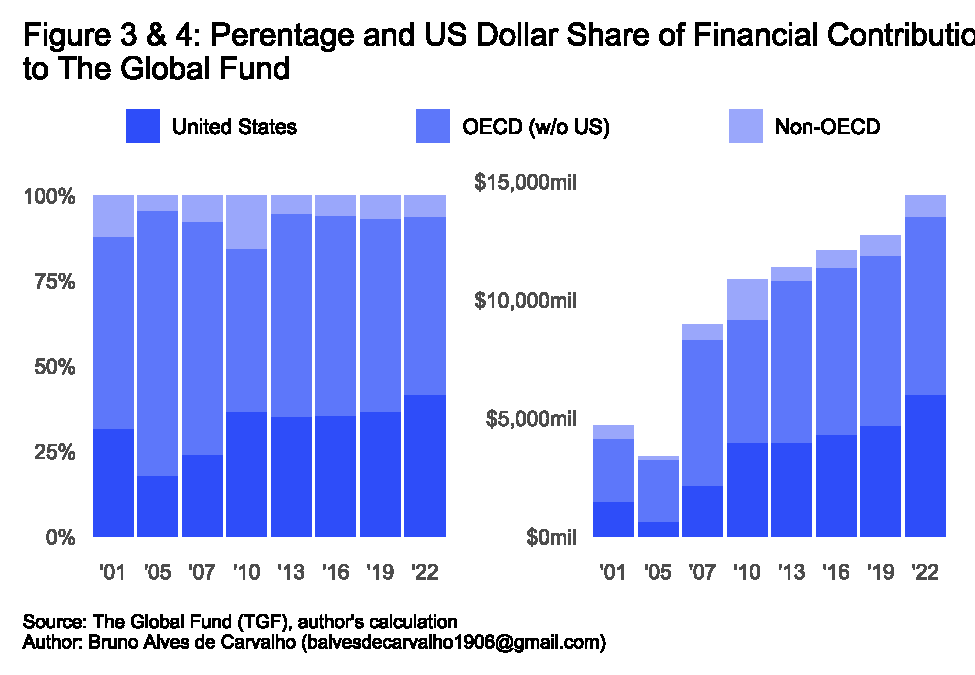
\includegraphics[keepaspectratio]{README_files/figure-latex/plot 3 & 4-1.pdf}}

Likewise, the number of public sector donors increased from 28 in 2013
to 36 in 2016, reaching 58 in 2019 and 49 in 2022 (see Figure 5). This
is higher than the initial group of public donors in 2001, who benefited
from the excitement surrounding the creation of this innovative
financing mechanism. Most new donors are low to middle-income countries,
reflecting a positive shift toward greater self-financing among
recipient nations.

However, despite this broader participation, contributions from new
donors remain relatively small, suggesting their pledges are more
intended to be symbolic commitments rather than financially
transformative. This means they cannot compensate for potential
reductions from major donors like the US and key European countries.
Additionally, while the number of donors has increased, the median
pledge per country has declined, from US\$46.2 million in 2013 to US\$10
million in 2022 (see Figure 6). This underscores a critical point:
increasing the number of donors alone is not enough to sustain overall
funding levels. To build a more resilient financial model, TGF must
attract a greater share of mid-sized donors, balancing its funding base
and reducing dependence on a single dominant donor\footnote{Exploring
  alternative funding sources beyond donors could also serve as a hedge
  against funding risks. This is particularly relevant for The Global
  Fund, which relies entirely on donor funding to finance its operations
  and investments. Such an approach might offer a more attractive hedge
  than attempting to expand the donor base, as the latter could become
  increasingly difficult in a world where globalization is retreating.
  There are already signs that the US may reduce funding to
  international organizations that receive financial support from China
  and other countries competing with America's global influence (Lynch,
  2025b).}.

Overall, the skewed distribution of pledges reveals deep structural
realities about international funding: economic disparities, donor
dominance, and long-term sustainability risks. Even though TGF has made
progress in diversifying its donor pool, the financial weight remains
highly concentrated among a few key players. These issues
notwithstanding, the Global Fund has benefited from consistent growth in
public sector funding, from US\$4.7 billion in 2001 to US\$14 billion in
2022, enabling it to improve health outcomes in developing countries and
earn international recognition. While the success of its grants has
undoubtedly played a role in securing continued support, other factors
may have also influenced public donor contributions. This question is
particularly relevant in an era when financing appears to be driven less
by the measurable impact of international aid and more by the alignment
of that aid with donor countries' national interests. In other words, we
must look beyond the effectiveness of aid programs and examine the
economic and political conditions shaping public donor contributions.

The extent of public sector pledges to The Global Fund can be understood
as a function of supply and demand. The demand for funding is
represented by current recipient country needs, as well as trends in the
incidence and mortality of HIV/AIDS, tuberculosis, and malaria (HTM).
Based on these factors, The Global Fund, in collaboration with academic
experts, has estimated that US\$18 billion is needed between 2027 and
2029 to stay on track to end HTM by 2030. On the supply side, a
country's ability and willingness to contribute money to the partnership
can be inferred from the overall pool of funds allocated for foreign
aid. One way to assess this is through trends in Official Development
Assistance (ODA), which reflect the total volume of aid disbursed by
donor countries. Higher ODA levels may indicate a greater likelihood of
increased contributions to The Global Fund. Similarly, if other
international aid organizations receive greater public sector
contributions, The Global Fund may also benefit, given that these
organizations operate within the same sector and under similar funding
conditions.

More fundamentally, the extent to which the supply of funds matches
demand depends on the broader political and economic context of donor
countries. For example, a government experiencing strong economic growth
and fiscal stability may be better positioned to contribute than one
facing recession and high public debt. Political ideology may also play
a role: left-leaning governments, which typically emphasize universal
healthcare and poverty reduction, may be more inclined to support
humanitarian initiatives, whereas right-leaning governments may
prioritize domestic spending and military investments. Additionally,
electoral cycles could impact funding commitments. During an election
year, governments may be preoccupied with domestic politics, making it
harder for The Global Fund to make its investment case heard.

Nonetheless, some governments may still maintain or even increase
contribut¨ions due to pre-existing commitments or a desire to uphold
international credibility, regardless of political and economic
conditions.

\pandocbounded{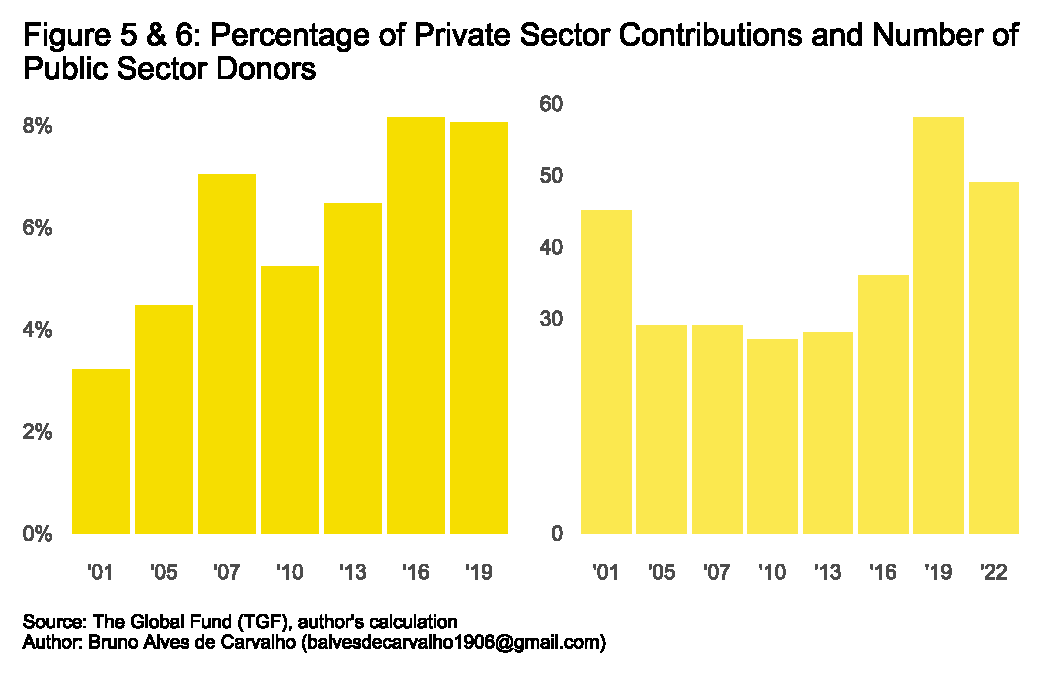
\includegraphics[keepaspectratio]{README_files/figure-latex/plot 5 & 6-1.pdf}}

\pandocbounded{\includegraphics[keepaspectratio]{README_files/figure-latex/plot 7-1.pdf}}

The generalizations outlined above may not apply universally. These
considerations form the basis of six hypotheses that this research will
test using publicly available data from multiple reputable sources,
namely: the International Monetary Fund (IMF), the OECD, the Center for
Global Development (CGD), the Chapel Hill Expert Survey (CHES), the
Party Government in Europe Database (PAGED), the ParlGov project, and
the Manifesto Project database (MP).

Having analysed the historical replenishment outcomes of The Global Fund
and outlined our hypotheses, we will now dig deeper into the data to
test our assumptions, identify patterns and trends in donor behavior,
and attempt to model these behaviors to create a predictive framework
for estimating future funding outcomes. Following that, we will discuss
the implications of the findings and offer recommendations for the
future sustainability of The Global Fund, particularly in light of the
evolving political and economic challenges.

\subsection{Hypotheses}\label{hypotheses}

\begin{enumerate}
\def\labelenumi{\arabic{enumi}.}
\tightlist
\item
  If the financial contributions from government donors to other global
  health organizations, such as GAVI, and multilateral development
  banks, like the IDA, decline, then the financial contributions from
  public donors to The Global Fund (TGF) will decrease, because TGF
  tends to align its funding expectations with global trends in public
  health financing.
\item
  If the Official Development Assistance (ODA) disbursements of
  government donors decline, then the financial contributions from
  public donors to The Global Fund (TGF) will decrease, because TGF's
  funding is indirectly influenced by overall humanitarian aid trends.
\item
  If the fiscal outlook of government donors, measured \emph{inter lia}
  by rising public debt and deteriorating fiscal balances, worsens, then
  the financial contributions from government donors to The Global Fund
  (TGF) will decrease, because weaker fiscal health limits governments'
  ability to make discretionary international contributions.
\item
  If the macroeconomic outlook of government donors, measured
  \emph{inter lia} by GDP growth and unemployment, worsens, then the
  financial contributions from government donors to The Global Fund
  (TGF) will decrease, because weaker economic growth limits
  governments' ability to make discretionary international
  contributions.
\item
  If the ideological placement of government donors, measured by their
  political and / or economic orientation, leans to the right, then the
  financial contributions from public donors to The Global Fund (TGF)
  will decrease, because right-wing governments tend to prioritize
  fiscal discipline and are less ideologically aligned with humanitarian
  spending.
\item
  If the replenishment year coincides with the re-election year of donor
  governments, then their financial contributions to The Global Fund
  (TGF) will be smaller, because electoral priorities and domestic
  political considerations may reduce focus on international aid
  commitments and make it more challenging for TGF to secure funding.
\end{enumerate}

\subsection{Hypotheses Testing}\label{hypotheses-testing}

The Global Fund is part of an ecosystem of international health
organizations, each playing a crucial role in combating HTM in low to
middle income countries. For instance, while TGF might finance the
purchase of health products, it relies on other partners to store,
transport, and administer these products to affected communities. This
interconnected network means that the success or failure of one
organization can significantly impact the others.

We can reasonably assume that this interdependence extends to financing.
Most global health organizations depend on ODA to fund their programs
and staff worldwide. Additionally, they often rely on the same group of
wealthy donors, though the degree of dependence may vary. As a result,
the funding levels received by other international aid organizations
might serve as a useful benchmark for the funding TGF receives during
its replenishments.

To test this assumption, we used data collected by the CGD on the
country pledges received by various Multilateral Development Banks
(MDBs) or concessional funds, such as the International Development
Association (IDA) of the World Bank, health funds like GAVI and the
Coalition for Epidemic Preparedness Innovations (CEPI), and climate
funds over the past two decades. By comparing these pledges with
contributions received by The Global Fund between 2001 and 2022, we
found a strong positive correlation across all organizations. While the
data is more limited for recently established entities like the Green
Climate Fund (GCF) and CEPI, the overall trend holds (see Figure 8).
This suggests that The Global Fund's replenishment outcomes are closely
aligned with those of other major multilateral funds, implying that when
donors increase funding to GAVI, for instance, they are also likely to
increase funding to The Global Fund, and vice versa.

This strong relationship may indicate that public sector donors treat
their international aid portfolios holistically, viewing support for
different global priorities, such as health and climate, as
complementary rather than competing. In this way, global aid does not
appear to function as a zero-sum game, where increases to one fund
necessarily mean cuts to another. Instead, donor behavior seems to
follow a ``win-win'' or ``loss-loss'' pattern: when overall aid budgets
grow, many multilateral organizations benefit, and when budgets shrink,
several are affected simultaneously. In today's climate of constrained
aid budgets, the critical question may be not whether funding will fall,
but which organizations will bear the greater burden.

Financial contributions to The Global Fund are also strongly and
positively correlated with the levels of ODA disbursements by public
sector donors. This relationship is expected, as ODA represents the main
financial channel through which governments support the economic
development and welfare of low and middle income countries, and The
Global Fund serves as a key multilateral mechanism through which donors
fulfill these commitments in the health sector. Therefore, the more a
country spends on ODA, the more we can typically expect it to contribute
to The Global Fund. Conversely, if a country's overall ODA spending
declines, its contributions to The Global Fund are also likely to fall.

Importantly, the strength of this relationship may vary depending on a
government's preference for bilateral versus multilateral aid. If a
country primarily delivers aid through bilateral channels, changes to
its ODA envelope may have a more limited impact on The Global Fund
compared to countries that prioritize multilateral mechanisms.

Beyond the direct supply of funding to aid organizations and recipient
countries through ODA, the economic and political context of donor
countries is also expected to play an important role in shaping
contributions to The Global Fund. Government pledges must ultimately be
financed through domestic tax revenue or borrowing. As such, a country's
tax capacity and its ability or willingness to raise debt can enable or
constrain its potential to supply ODA, and, by extension, its ability to
fund global health initiatives like The Global Fund. However, it is
important to note that ODA levels are not determined solely by fiscal
space; they often reflect political priorities and strategic choices.

The IMF regularly compiles data to monitor the fiscal health of
governments around the world. Its Fiscal Monitor includes eight
standardized indicators (as percentages of GDP): government expenditure,
government revenue, (primary) net lending / borrowing, gross debt, net
debt, and cyclically adjusted (primary) balance. These measures gauge
whether a government is operating within prudent fiscal limits or
running into fiscal strain.

By mapping these fiscal metrics against donor contributions to The
Global Fund, we find that pledges exhibit a weak negative correlation
with indicators of fiscal balance. When looking at the overall fiscal
stance without adjusting for the economic cycle, the correlation between
fiscal balance and contributions is very weak, suggesting there may be
no meaningful relationship between the two. However, when we isolate the
structural fiscal position by removing cyclical effects, the correlation
strengthens slightly, though it remains weak overall.

\pandocbounded{\includegraphics[keepaspectratio]{README_files/figure-latex/plot 8-1.pdf}}

\pandocbounded{\includegraphics[keepaspectratio]{README_files/figure-latex/plot 9-1.pdf}}

This points to a tentative trend: donor countries that are structurally
more fiscally conservative, or that operate under tighter long-term
budgetary constraints, tend to pledge less to The Global Fund than those
with less sustainable levels of public debt.

This pattern is further supported by the weak positive correlation
observed between government debt levels and financial contributions to
The Global Fund. When examining the total stock of government debt, or
gross debt, we find a moderate correlation with TGF pledges, indicating
that countries with higher debt burdens are not necessarily limited in
their ability to provide aid, and may actually be more inclined to
pledge generously. However, when we shift focus to net debt, adjusting
for government financial assets, the correlation weakens. This is likely
because government assets are often illiquid or politically constrained,
and therefore do not directly translate into available or discretionary
resources for development assistance. In other words, while gross debt
may reflect a broader willingness to rely on debt-financed spending, net
debt offers less insight into a government's real-time capacity or
political inclination to fund The Global Fund.

At first, it may seem counterintuitive that countries with higher debt
burdens might also contribute more to The Global Fund. Instead, one
might expect highly indebted countries to reduce discretionary spending,
such as aid, in an effort to repair their balance sheets. However,
countries that are more comfortable financing public spending through
debt may, paradoxically, have greater fiscal space to maintain or even
increase aid commitments. Some high-income countries enjoy strong credit
ratings and low borrowing costs, giving them more flexibility to sustain
international commitments, including ODA. In this context, global health
spending can be viewed not as a financial burden, but as a strategic
investment aligned with foreign policy and soft power objectives.

Countries with stronger fiscal balances may also be constrained by
domestic rules or political pressures. For example, Germany's ``debt
brake'' limits the federal deficit to 0.35\% of GDP. Switzerland has a
similar mechanism that caps spending based on cyclical economic
performance. In such settings, even when fiscal capacity exists, legal
or political constraints may prevent governments from increasing
international aid. Much like the US, recent budget cuts to foreign aid
in the Netherlands have been justified under a ``Netherlands-first''
approach, highlighting that political will, not just fiscal capacity,
often determines aid decisions.

Finally, the data also shows that donor pledges are weakly and
positively correlated with levels of government expenditure and revenue.
This aligns broadly with our previous observations, as we might expect
governments that spend more to carry higher debt burdens and often
exhibit weaker fiscal balances. Similarly, countries with greater
capacity to raise revenue through taxation may have more fiscal space to
allocate towards global health, even if higher revenues are typically
associated with more balanced budgets and lower debt levels.

What makes this finding particularly interesting is that it suggests
donors are willing to mobilize either their own funds or borrowed
resources to finance multilateral initiatives like The Global Fund.
Although our analysis does not track whether TGF pledges are financed
through debt or taxes, the patterns suggest that, for some governments,
sovereign debt may serve as a flexible policy instrument, enabling them
to support TGF when it aligns with broader diplomatic, humanitarian, or
geopolitical goals, rather than requiring trade-offs with domestic
spending. For others, financial contributions to The Global Fund may
represent a relatively minor share of total revenue, small enough to
absorb without the need to incur additional debt.

To explore how broader macroeconomic conditions might affect public
sector funding, we examined macroeconomic indicators using data from the
IMF's World Economic Outlook. These include GDP (\%) change and GDP per
capita, inflation, unemployment, trade, and investment levels. One of
our initial assumptions was that a strong economic outlook would
positively influence financial contributions to The Global Fund.

{[}Integrate better{]} One notable trend is the weak positive
correlation between pledges and GDP per capita. As a rough proxy for
individual wealth and a country's level of development, GDP per capita
helps explain why wealthier countries tend to contribute more to The
Global Fund. This is consistent with the Fund's donor profile, which is
largely composed of high-income countries with greater fiscal space to
support multilateral health efforts.

While we find a weak negative correlation between unemployment and
pledges, suggesting that countries experiencing rising unemployment may
be slightly less inclined to contribute, likely due to fiscal pressures
from lower tax revenues and higher welfare spending, the rest of the
relationships paint a more nuanced picture.

Interestingly, the rate of GDP growth appears to be negatively
correlated with pledges. This counterintuitive trend likely reflects the
composition of TGF's donor base: countries that have seen rapid economic
growth, say above 6\% annually, over the past two decades are
predominantly emerging or developing economies, which are not major
contributors to the Fund. In contrast, the largest donors, such as the
US, Japan, Germany, and France, have experienced more modest growth
during the same period, which may help explain this inverse
relationship.

This trend is mirrored by the positive relationship between GDP per
capita and pledges. As a rough proxy for individual wealth and a
country's level of development, GDP per capita helps illustrate why
wealthier countries tend to contribute more to The Global Fund. This is
consistent with the Fund's donor profile, which is largely composed of
high-income countries with greater fiscal space to support multilateral
health efforts.

Additionally, inflation shows a weak negative correlation with pledges.
Even though moderate inflation can accompany economic growth, high
inflation often reflects economic instability or policy uncertainty. For
donors, high inflation may erode the real value of contributions or
signal a fragile economic environment, leading them to scale back or
delay pledges.

When examining total investment levels, often viewed as an indicator of
domestic confidence in future growth, we observe no significant
correlation with donor pledges. This suggests that domestic economic
optimism does not necessarily translate into higher international aid
commitments to The Global Fund. Likewise, the negative relationship
between pledges and trade volume suggests that increasing trade activity
is not a strong driver of donor generosity. Many emerging economies with
rapidly rising trade integration are not primary contributors to The
Global Fund, while traditional donors with slower trade growth possess
greater fiscal capacity to fund the partnership.

\pandocbounded{\includegraphics[keepaspectratio]{README_files/figure-latex/plot 10-1.pdf}}

\pandocbounded{\includegraphics[keepaspectratio]{README_files/figure-latex/plot 11-1.pdf}}

In sum, across all key macroeconomic indicators analyzed, we observe
weak to no correlations with Global Fund pledges. This suggests that
while economic conditions may shape the broader fiscal landscape, they
are not strong predictors of donor behavior toward TGF. Indeed, there is
some historical evidence supporting this. During the 2008 Global
Financial Crisis, while many governments cut or postponed some domestic
spending, aggregate levels of ODA held relatively steady. Donor
commitments to The Global Fund, in fact, continued to rise in nominal
terms between 2007 and 2016 (see Figure 4). This resilience indicates
that global health funding may be shielded, at least in the short term,
from economic shocks.

There are multiple reasons for this. Many donor governments treat global
health as a moral or diplomatic priority, and multilateral platforms
like The Global Fund encourage burden-sharing and peer accountability.
As a result, a country might sustain or increase pledges based on prior
rounds of funding even during periods of economic weakness to maintain
international credibility or signal leadership in global health.

This underscores the importance of political context in shaping the
level of funding The Global Fund receives. Though political dynamics are
inherently fluid and difficult to quantify, we will try to examine their
potential influence through a set of commonly held views. A common
belief is that left-leaning governments, being more aligned with
humanitarian values, are more inclined to support international aid. A
notable example is the Biden administration, whose progressive agenda
included a strong commitment to global health, and to The Global Fund in
particular. Similarly, commentators often express concern when
replenishments coincide with election periods in key donor countries,
fearing that governments may prioritize re-election campaigns over
global health commitments. On the surface, both assumptions seem
reasonable.

To explore these dynamics, we compiled historical data on the
ideological orientation of major democratic donors to The Global Fund,
drawing from four key databases. The Chapel Hill Expert Survey (CHES)
provides expert assessments of party positions across Europe; PAGED
tracks party participation in executive office globally since 1990;
ParlGov links information on elections, political parties, and
governments in parliamentary systems; and the Manifesto Project analyzes
party manifestos to quantify ideological positions and policy priorities
over time.

Surprisingly, the data indicates a weak but positive relationship
between the ideological placement of donor governments and their
financial pledges to The Global Fund. This suggests that right-leaning
governments tend to pledge slightly more slightly more on average,
though not consistently or reliably, than left-leaning ones. Economic
ideology appears to correlate more strongly with pledges than overall
political ideology, implying that funding levels may be more closely
tied to governments' economic priorities than their overall political
orientation. However, the weakness of these correlations means that
ideology alone is not a strong or consistent predictor of donor
behavior.

Indeed, historical examples challenge conventional assumptions. It was
the conservative Republican Bush administration that launched the
President's Emergency Plan for AIDS Relief (PEPFAR), one of the largest
bilateral health initiatives in history. Many right-leaning governments
in the 2000s and 2010s actively supported the liberal, rules-based
international order that fostered multilateral initiatives like The
Global Fund, though this was equally true for many left-leaning
governments. In fact, The Global Fund has traditionally enjoyed broad
bipartisan support. For example, the first Trump administration not only
maintained support for the Fund but increased the U.S. contribution in
2019. More broadly, parliamentary democracies like Germany or the UK can
blur ideological lines as budget and foreign aid decisions might reflect
consensus rather than partisan ideology, further weakening the
ideological link.

These examples suggest that a simplistic left-to-right ideological
framework may not offer a reliable heuristic for predicting public
sector pledges. Political ideologies are fluid and evolve over time. In
the current landscape, we have even seen former champions of
multilateralism, like the U.S. Republican Party, take a more adversarial
stance toward the liberal international order they once helped shape.

A more useful political factor influencing contributions to The Global
Fund may be the timing of domestic elections. The data shows that the
median pledge decreases significantly, from \$184 million to \$99
million, when replenishment periods overlap with national elections.
While this correlation is also weak, the trend may reflect several
plausible dynamics: elections can cause administrative delays, lead to
fiscal caution as governments avoid new spending commitments, and
trigger shifts in political attention toward domestic

\pandocbounded{\includegraphics[keepaspectratio]{README_files/figure-latex/plot 12-1.pdf}}

\pandocbounded{\includegraphics[keepaspectratio]{README_files/figure-latex/plot 13-1.pdf}}

priorities that resonate more strongly with voters. These factors may
collectively reduce the bandwidth and willingness of governments to make
ambitious international pledges during electoral periods.

So far, the analysis suggests that several commonly held assumptions do
not fully hold up under scrutiny. While pledges to The Global Fund are
strongly correlated with overall ODA levels and with contributions to
other multilateral development organizations, and while domestic
elections in donor countries appear to have a dampening effect on
pledges, we find little evidence that a donor's fiscal or macroeconomic
outlook is strongly associated with higher contributions. Likewise,
widely held beliefs about the influence of political ideology on donor
generosity have also been called into question.

Nonetheless, to rigorously test these relationships, we need to take the
analysis a step further by modeling them mathematically through
regression analysis. This approach allows us to assess the influence of
individual factors, such as fiscal metrics, political ideology, or
economic conditions, while controlling for other variables
simultaneously. In doing so, we can better isolate the specific impact
of each factor and identify the drivers of financial contributions to
The Global Fund.

Regression analysis also enables us to evaluate the reliability of our
observations by testing their statistical significance and goodness of
fit. This helps us determine whether the relationships we have
identified are likely to hold beyond past replenishment outcomes, making
them applicable to future replenishments. Finally, assuming we are able
to build a robust model that captures the key predictors of public
sector pledges, we may even be able to generate informed projections of
future funding outcomes.

\subsection{Recommendations}\label{recommendations}

Development assistance for health peaked in 2021 at US\$84 billion with
the COVID-19 pandemic. Return to pre-pandemic levels of funding is
already underway, levels of financing could fall farther below if donors
reallocate development assistance away from health due to other
priorities like war or climate change. At best, health funding is
regressing to the mean.

\subsection{Methodolgy}\label{methodolgy}

Before modeling, I performed some anticipatory transformations to the
data. We used the US Federal Reserve Bank's price deflator to transform
nominal dollar pledges into 2022 constant prices to limit the impact of
currency fluctuations on the model. Additionally, we created a new
variable calculating the average donor pledge to each development
organization in our sample. This helped limit the impact of colinearity
in the final model. We did the same with the different measures of party
ideological orientation. Finally, we calculated the log of each dollar
denominated variable to improve model performance. For economic
indicators, we calculated the 3-year rolling average to account for the
effect of previous economic performance on donor pledges during the
replenishment year.

Important to ask which model to use. Multiple are available. For sake of
practicality, and given our small sample size (n = 141), I decided to
opt for a multiple linear regression, over a multi-level model, which
might have better modeled the structural nature of the data, though it
may have under-performed due to the small number of donor observations.
A multilevel model typically requires n observations per unit and n
number of units to function properly (citation).

Thankfully, it is possible to account for the fixed-effects of the donor
countries in a multiple linear regression by including the donor
variable in the model, as well as the value of the replenishment year.
This will help off-set the impact of country and time specific effects
on the other coefficients, allowing us to have a cleaner view of the
actual impact of predictors on the outcome of the replenishment.

However, the introduction of donor countries as a control variable
increases the number of variables in our model, as each donor country is
represented as a separate variable in the model. The reliability of a
model can be negatively impacted when the number of predictors is large
in comparison to the number of observations. Moreover, we are including
many predictors that may not have any relation with donor pledges, and
including them may create unnecessary complexity in the resulting model.

For these reasons, I used two methods to manage these issues: forward
stepwise selection and shrinkage. The former involves beginning with a
model containing no predictors and then adding one predictor at a time,
starting with the predictor that gives the greatest additional
improvement to the fit. The objective being to identify the model with a
subset of the predictors that performs best against the test data. The
latter involves shrinking the predictors towards zero and identifying
the level of shrinkage that performs best against the test data. This is
a well known technique used to mitigate high variance, which can help
improve the reliability of a model. There two best-known shrinkage types
are the ridge regression and the lasso. We used both but have a
preference for the lasso because it has the added advantage of
performing variable selection by actually shrinking irrelevant
predictors to exactly zero, hence facilitating the interpretation of the
model results. Additionally, we have reasons to believe the lasso will
perform better than the ridge regression because our descriptive
analysis has shown that donor pledges seem to be strongly associated
with a small subset of predictors, namely the amount spend on ODA and
the financial contribution to other international development
organizations like The Global Fund.

To compare the performance of these three different modeling techniques,
we used a re-sampling method known as cross-validation. This involves
repeatedly drawing a sample of the data, refitting the model on each
sample, and testing each model on the rest of the data. In other words,
cross-validation involves randomly dividing the data into a training and
validation set, allowing us to assess the performance of a model trained
on the training set and tested on the validation set. The purpose of
cross-validation is to simulate real life. Instead of fitting the model
on the whole data from the start, we can learn a great deal about how
accurate and reliable our model is likely to be by training it on a
sample of our data and testing it on ``new'' data, that is, the data we
left out. The challenge of many statistical models based on a sample of
a wider population is generalizability: will your model behave the same
with new data? The cross-validation approach allows us to mimic this.

We opted for a 5-fold cross-validation, randomly splitting observations
into five non-overlapping validation groups. After running each model,
we compared them using the Mean Squared Error (MSE), a measure of the
validation set error rate, that is, how close the model predictions
match the actual pledges of the new test data. The smaller the MSE the
better. Before jumping into the cross-validation results, it is
important to note that we excluded the control variables, namely the
donor countries and the replenishment year, from this initial phase of
the variable selection process. This is because all control variables
need to be included in the final model, regardless of their
significance, if we want to control for country and time specific noises
in the data.

The results show that the multiple linear regression, or OLS (for
Ordinary Least Squares), performed on average better than the ridge
regression and lasso when fitted against the validation set. The ridge
regression performed the least well, with the lasso performing bang in
the middle. At first, this shows that a full model like the ridge
regression, even if it shrinks predictors, tends to underperform against
models that select a subset of predictors. Additionally, it doesn't seem
like the shrinkage, whether in the ridge or lasso, provides an edge over
the multiple linear regression combined with stepwise selection.

\begin{longtable}[]{@{}rrr@{}}
\caption{Table 1: Mean Squared Error by Model}\tabularnewline
\toprule\noalign{}
OLS & Ridge & Lasso \\
\midrule\noalign{}
\endfirsthead
\toprule\noalign{}
OLS & Ridge & Lasso \\
\midrule\noalign{}
\endhead
\bottomrule\noalign{}
\endlastfoot
0.67 & 0.73 & 0.7 \\
\end{longtable}

If we examine which variables were included in the OLS model with the
lowest MSE in each fold, we observe that, 5 out of 5 times, the model
contains the value spent on ODA and the financial contributions to other
development organizations by donor countries. Other economic and
political factors are also included, but less often. Some variables are
behaving strangely as compared to our descriptive analysis, though. We
did not expect the unemployment rate to be positively related to
pledges, neither did we expect the \% change in GDP to be positively
associated with pledges, even though this was our initial hypothesis.

\begin{longtable}[]{@{}lrr@{}}
\caption{Table 2: Predictors Included in Best OLS model}\tabularnewline
\toprule\noalign{}
Variable & Included & Mean\_Coef \\
\midrule\noalign{}
\endfirsthead
\toprule\noalign{}
Variable & Included & Mean\_Coef \\
\midrule\noalign{}
\endhead
\bottomrule\noalign{}
\endlastfoot
oda\_spent\_log & 5 & 0.7540442 \\
other\_orgs\_cp\_log & 5 & 0.6595083 \\
gdp\_cp\_rllavg02 & 3 & 0.1084560 \\
gdp\_per\_cap\_cp\_log\_rllavg02 & 1 & 0.6245307 \\
yes\_elec & 1 & -0.2664715 \\
unemployment\_rt\_rllavg02 & 1 & 0.0891353 \\
\end{longtable}

Interestingly, the six variables included in one or more of the best OLS
models correspond with the top six stronger predictors in the ridge
regression and lasso (see table 3 and 4), though the lasso tends to
include more variables in more of its models than the OLS. Each of these
six predictors also seem to be behaving in the same direction. This
leads us to think that the final model would have to include either all
or at least some of these six variables: ODA disbursements, financial
contributions to other development organizations, GDP per Capita, \%
Change in GDP, election year, and the unemployment rate.

\begin{longtable}[]{@{}lr@{}}
\caption{Table 3: Predictors Included in Best Ridge
Regression}\tabularnewline
\toprule\noalign{}
Variable & Mean\_Coef \\
\midrule\noalign{}
\endfirsthead
\toprule\noalign{}
Variable & Mean\_Coef \\
\midrule\noalign{}
\endhead
\bottomrule\noalign{}
\endlastfoot
oda\_spent\_log & 0.7034599 \\
other\_orgs\_cp\_log & 0.6329802 \\
gdp\_per\_cap\_cp\_log\_rllavg02 & 0.4687356 \\
yes\_elec & -0.2252039 \\
gdp\_cp\_rllavg02 & 0.0874203 \\
unemployment\_rt\_rllavg02 & 0.0620298 \\
adjfsclblc\_rllavg01 & -0.0241781 \\
imports\_vl\_rllavg02 & 0.0234048 \\
Total\_investment\_rllavg02 & -0.0207480 \\
lr\_all & 0.0192702 \\
prmryfsclblc\_rllavg01 & 0.0171899 \\
prmryadjfsclblc\_rllavg01 & 0.0140604 \\
inflation\_rt\_rllavg02 & 0.0113104 \\
exports\_vl\_rllavg02 & -0.0101360 \\
grsdbt\_rllavg01 & 0.0030844 \\
expdtr\_rllavg01 & -0.0016318 \\
revn\_rllavg01 & -0.0014241 \\
fsclblc\_rllavg01 & -0.0010522 \\
ntdbt\_rllavg01 & -0.0009877 \\
\end{longtable}

\begin{longtable}[]{@{}lrr@{}}
\caption{Table 4: Predictors Included in Best Lasso}\tabularnewline
\toprule\noalign{}
Variable & Included & Mean\_Coef \\
\midrule\noalign{}
\endfirsthead
\toprule\noalign{}
Variable & Included & Mean\_Coef \\
\midrule\noalign{}
\endhead
\bottomrule\noalign{}
\endlastfoot
oda\_spent\_log & 5 & 0.7208286 \\
other\_orgs\_cp\_log & 5 & 0.6552166 \\
gdp\_cp\_rllavg02 & 5 & 0.0684934 \\
unemployment\_rt\_rllavg02 & 5 & 0.0455947 \\
gdp\_per\_cap\_cp\_log\_rllavg02 & 4 & 0.2440381 \\
yes\_elec & 4 & -0.1685914 \\
lr\_all & 3 & 0.0027206 \\
imports\_vl\_rllavg02 & 2 & 0.0296070 \\
Total\_investment\_rllavg02 & 2 & -0.0231038 \\
inflation\_rt\_rllavg02 & 2 & -0.0191062 \\
prmryadjfsclblc\_rllavg01 & 2 & 0.0030300 \\
grsdbt\_rllavg01 & 2 & 0.0007513 \\
prmryfsclblc\_rllavg01 & 1 & 0.0174462 \\
adjfsclblc\_rllavg01 & 1 & -0.0086971 \\
\end{longtable}

The variable selection conducted by the lasso has the advantage of being
less restrictive than the one done by the OLS, without necessarily
sacrificing too much predictive accuracy. It is therefore worth keeping
it for the moment, unlike the ridge regression which includes all
variables but suffers from the lowest predictive accuracy.

We will now run the OLS and lasso models again with the control
variables and compare their output. Variables selected at least once in
the previous OLS are included in this new regression model. The lasso is
run on all predictors again, but this time including the control
variables.

Examining the lasso first, (compare coefficients between OLS and Lasso).

\begin{longtable}[]{@{}lr@{}}
\caption{Table 7:}\tabularnewline
\toprule\noalign{}
Variable & Coef \\
\midrule\noalign{}
\endfirsthead
\toprule\noalign{}
Variable & Coef \\
\midrule\noalign{}
\endhead
\bottomrule\noalign{}
\endlastfoot
oda\_spent\_log & 0.6024546 \\
other\_orgs\_cp\_log & 0.3784998 \\
yes\_elec & -0.0978967 \\
adjfsclblc\_rllavg01 & -0.0869754 \\
prmryfsclblc\_rllavg01 & 0.0785729 \\
gdp\_cp\_rllavg02 & -0.0564813 \\
inflation\_rt\_rllavg02 & -0.0531607 \\
unemployment\_rt\_rllavg02 & -0.0492652 \\
lr\_all & 0.0432843 \\
exports\_vl\_rllavg02 & 0.0012277 \\
\end{longtable}

\begin{longtable}[]{@{}lr@{}}
\caption{Table 6:}\tabularnewline
\toprule\noalign{}
Variables & Coef \\
\midrule\noalign{}
\endfirsthead
\toprule\noalign{}
Variables & Coef \\
\midrule\noalign{}
\endhead
\bottomrule\noalign{}
\endlastfoot
oda\_spent\_log & 0.6259517 \\
other\_orgs\_cp\_log & 0.3647519 \\
gdp\_cp\_rllavg02 & -0.0509000 \\
gdp\_per\_cap\_cp\_log\_rllavg02 & 0.7677343 \\
yes\_elec & -0.1149611 \\
unemployment\_rt\_rllavg02 & -0.0421040 \\
\end{longtable}

\begin{verbatim}
## Warning: Removed 513 rows containing missing values or values outside the scale range
## (`geom_line()`).
\end{verbatim}

\begin{verbatim}
## Warning: Removed 570 rows containing missing values or values outside the scale range
## (`geom_line()`).
\end{verbatim}

\pandocbounded{\includegraphics[keepaspectratio]{README_files/figure-latex/table 5 and plot-1.pdf}}

We basically end up with two final models with a subset of predictors,
one achieved through forward step-wise selection and the other via the
lasso.

This is a micro analysis, so focus on The Global Fund (over ODA and
Global Health as such). Basically, don't mix macro into a micro
analysis. Make sure you stay grounded in your data.

\subsection{Sources}\label{sources}

Apeagyei (Micah), A., Dieleman, J. and Leach-Kemon, K. (2024) Financing
Global Health 2023: The Future of Health Financing in the Post-Pandemic
Era. Institute for Health Metrics and Evaluation, 14 May. Available at:
\url{https://www.healthdata.org/research-analysis/library/financing-global-health-2023-future-health-financing-post-pandemic-era}
(Accessed: 1 April 2025).

Döring, H. and Manow, P. (2024) ParlGov 2024 Release. Available at:
\url{https://doi.org/10.7910/DVN/2VZ5ZC} (Accessed: 22/03/2025).

Galvin, G. (2025) `\,``Utterly devastating'': Global health groups left
reeling as European countries slash foreign aid', Euronews, 7 March.
Available at:
\url{https://www.euronews.com/health/2025/03/07/utterly-devastating-global-health-groups-left-reeling-as-european-countries-slash-foreign-}
(Accessed: 23 March 2025).

Hellström, J., Bergman, T., Lindahl, J. and Gustafsson, E.K. (2025) The
Representative Democracy Data Archive (REPDEM) -- Basic dataset, Version
2025.03. Available at: \url{https://repdem.org} (Accessed: 22/03/2025).

International Monetary Fund (IMF) (2024) Fiscal Monitor (FM) Dataset.
Available at:
\url{https://betadata.imf.org/en/Data-Explorer?datasetUrn=IMF.FAD:FM(5.0.0})
(Accessed: 22/02/2025).

International Monetary Fund (IMF) (2024) World Economic Outlook (WEO)
Database, October 2024. Available at:
\url{https://www.imf.org/en/Publications/WEO/weo-database/2024/October}
(Accessed: 22/03/2025).

Jerving, S. (2025a) `Scoop: UN migration agency cuts more jobs, shutters
lifesaving programs', Devex, 20 March. Available at:
\url{https://www.devex.com/news/memo-lays-out-plan-to-replace-usaid-with-new-humanitarian-agency-109685}
(Accessed: 22 March 2025).

Jerving, S. (2025b) `Memo lays out plan to replace USAID with new
humanitarian agency', Devex, 20 March. Available at:
\url{https://www.devex.com/news/memo-lays-out-plan-to-replace-usaid-with-new-humanitarian-agency-109685}
(Accessed: 23 March 2025).

Jolly, S., Bakker, R., Hooghe, L., Marks, G., Polk, J., Rovny, J.,
Steenbergen, M. and Vachudova, M.A.~(2022) `Chapel Hill Expert Survey
Trend File, 1999-2019', Electoral Studies, 75 (February). Available at:
\url{https://doi.org/10.1016/j.electstud.2021.102420} (Accessed:
22/03/2025).

Lehmann, P., Franzmann, S., Al-Gaddooa, D., Burst, T., Ivanusch, C.,
Regel, S., Riethmüller, F., Volkens, A., Weßels, B. and Zehnter, L.
(2024) The Manifesto Data Collection. Manifesto Project
(MRG/CMP/MARPOR). Version 2024a. Berlin: Wissenschaftszentrum Berlin für
Sozialforschung (WZB) / Göttingen: Institut für Demokratieforschung
(IfDem). Available at:
\url{https://doi.org/10.25522/manifesto.mpds.2024a} (Accessed:
22/03/2025).

Lynch, C. (2025a) `Exclusive: UN Refugee Agency braces for thousands of
job cuts', Devex, 20 March. Available at:
\url{https://www.devex.com/news/exclusive-un-refugee-agency-braces-for-thousands-of-job-cuts-109693}
(Accessed: 22 March 2025).

Lynch, C. (2025b) `Trump's new `loyalty test' for UN and aid groups',
Devex, 12 March. Available at:
\url{https://www.devex.com/news/trump-s-new-loyalty-test-for-un-and-aid-groups-109635}
(Accessed: 23 March 2025).

Madan Keller, J., Landers, C., Martinez, N. and Eldridge, R. (2024) `The
2024--2025 replenishment traffic jam', Center for Global Development, 16
October. Available at:
\url{https://www.cgdev.org/media/2024-2025-replenishment-traffic-jam}
(Accessed: 22/03/2025).

Ravelo, J.L. (2025a) `Stop TB Partnership looks at downsizing after
USAID cuts', Devex, 4 March. Available at:
\url{https://www.devex.com/news/stop-tb-partnership-looks-at-downsizing-after-usaid-cuts-109544}
(Accessed: 22 March 2025).

Ravelo, J.L. (2025b) `Exclusive: UNAIDS staff anxious as restructuring
looms amid aid cuts', Devex, 14 March. Available at:
\url{https://www.devex.com/news/exclusive-unaids-staff-anxious-as-restructuring-looms-amid-aid-cuts-109638}
(Accessed: 22 March 2025).

Rovny, J., Bakker, R., Hooghe, L., Jolly, S., Marks, G., Polk, J.,
Steenbergen, M. and Vachudova, M.A.~`25 Years of Political Party
Positions in Europe: The Chapel Hill Expert Survey, 1999-2024', working
paper.

The Global Fund (2025) The Global Fund Investment Case. Available at:
\url{https://www.theglobalfund.org/en/investment-case/} (Accessed:
22/03/2025).

Toosi, N. and Lippman, D. (2025) `Trump aides circulate plan for
complete revamp of foreign aid programs', Politico, 19 March. Available
at:
\url{https://www.politico.com/news/2025/03/19/trump-aides-circulate-plan-for-complete-revamp-of-foreign-aid-programs-00238862}
(Accessed: 23 March 2025).

\end{document}
